\lab{Python}{The Top-flight Trio}{The Top-flight Trio}
\label{Lab:PythonAdvanced}

\section*{NumPy + SciPy}
Numpy provides an extremely efficient, multidimensional array datatype.  Mastery of this array datatype will be invaluable in your journey through numerical computing with Python.  Without NumPy arrays, Python would be too slow to be an effective tool.  The secret is that NumPy arrays are actually thin wrappers around C arrays.  Arrays use zero-based indexing, just like the rest of Python.  Many of the operations on NumPy arrays are almost as fast as they would be in C.  SciPy is a more feature rich environment than NumPy, but uses the array datatype provided by NumPy.  In these labs, we will almost always exclusively use the SciPy library.

To make the SciPy library available for use, you must import it.  We prefer to import SciPy into its own namespace for cleaner, clearer code.
\begin{lstlisting}[style=python]
: import scipy as sp
\end{lstlisting}

The best way to conceptually think of NumPy arrays is to visualize nested arrays.  For a $3\times4$ matrix, think of an array that contains three arrays each of length four.  Let's practice with a three dimensional matrix.

\[
A = \begin{bmatrix}
\begin{bmatrix}
0 & 1 \\
2 & 3 \\
4 & 5 \\
6 & 7 \\
8 & 9
\end{bmatrix}
\begin{bmatrix}
10 & 11 \\
12 & 13 \\
14 & 15 \\
16 & 17 \\
18 & 19
\end{bmatrix}
\begin{bmatrix}
20 & 21 \\
22 & 23 \\
24 & 25 \\
26 & 27 \\
28 & 29
\end{bmatrix}
\end{bmatrix}
\]

NumPy tracks each dimension by an axis number, also starting at $0$.  A one dimensional array has only one axis, a two dimensional, two axis.  An $n$ dimensional array has $n$ axis.  Our three dimensional array has dimensions $(3,5,2)$.  If we wanted to retrieve the value $16$, we would need to first retrieve index $1$ in axis $0$.
\[
A[1] = \begin{bmatrix}
10 & 11 \\
12 & 13 \\
14 & 15 \\
16 & 17 \\
18 & 19
\end{bmatrix}
\]

Then we need to retrieve index $3$ in axis $1$.
\[
A[1,3] = \begin{bmatrix}
         16 & 17 \\
         \end{bmatrix}
\]

Then we retrieve index $0$ of axis $2$.
\[
A[1,3,0] = 16
\]

\subsection*{Manipulating Arrays}
Array operations are, by default, element wise.  This includes multiplying arrays.

\begin{lstlisting}[style=python]
: a = sp.array(range(9)).reshape(3,3)
#flip a left right and up down.  We make b an upside down and backwards copy of a
: b = sp.flipud(sp.fliplr(a))
: a + b
array([[8, 8, 8],
       [8, 8, 8],
       [8, 8, 8]])
: a * b #this is NOT matrix multiplication
array([[ 0,  7, 12],
       [15, 16, 15],
       [12,  7,  0]])
: sp.dot(a, b) #this is matrix multiplication
array([[ 9,  6,  3],
       [54, 42, 30],
       [99, 78, 57]])
\end{lstlisting}

Unlike Python lists, arrays are allocated upon creation and are not dynamic.  It is expensive to change the dimensions of an array after it has been allocated.  We will demonstrate this by adding columns to an array vs allocating the entire array and changing the elements.

\begin{lstlisting}[style=python]
def allocateAll(n):
    #allocate an nxn array
    A = sp.zeros((n,n))
    for a in xrange(n):
        for b in xrange(n):
            A[a, b] = sp.math.cos(a*b)
    return A

def appendOne(n):
    A = sp.array([])
    for a in xrange(n):
        for b in xrange(n):
	    A = sp.append(A, sp.math.cos(a*b))
    return A.reshape(n, n)
\end{lstlisting}

\begin{lstlisting}[style=python]
: import mytimer
: with mytimer.timer() as timer:
:     for x in xrange(1, 50):
:         timer.time(appendOne, x)
:         timer.time(allocateAll, x)
: #let's plot the results
: import matplotlib.pyplot as plt
: sizes = range(1,50)
: plt.plot(sizes, timer.results['appendOne'], 'r')
: plt.plot(sizes, timer.results['allocateAll'], 'b')
: plt.show()
\end{lstlisting}

\begin{center}
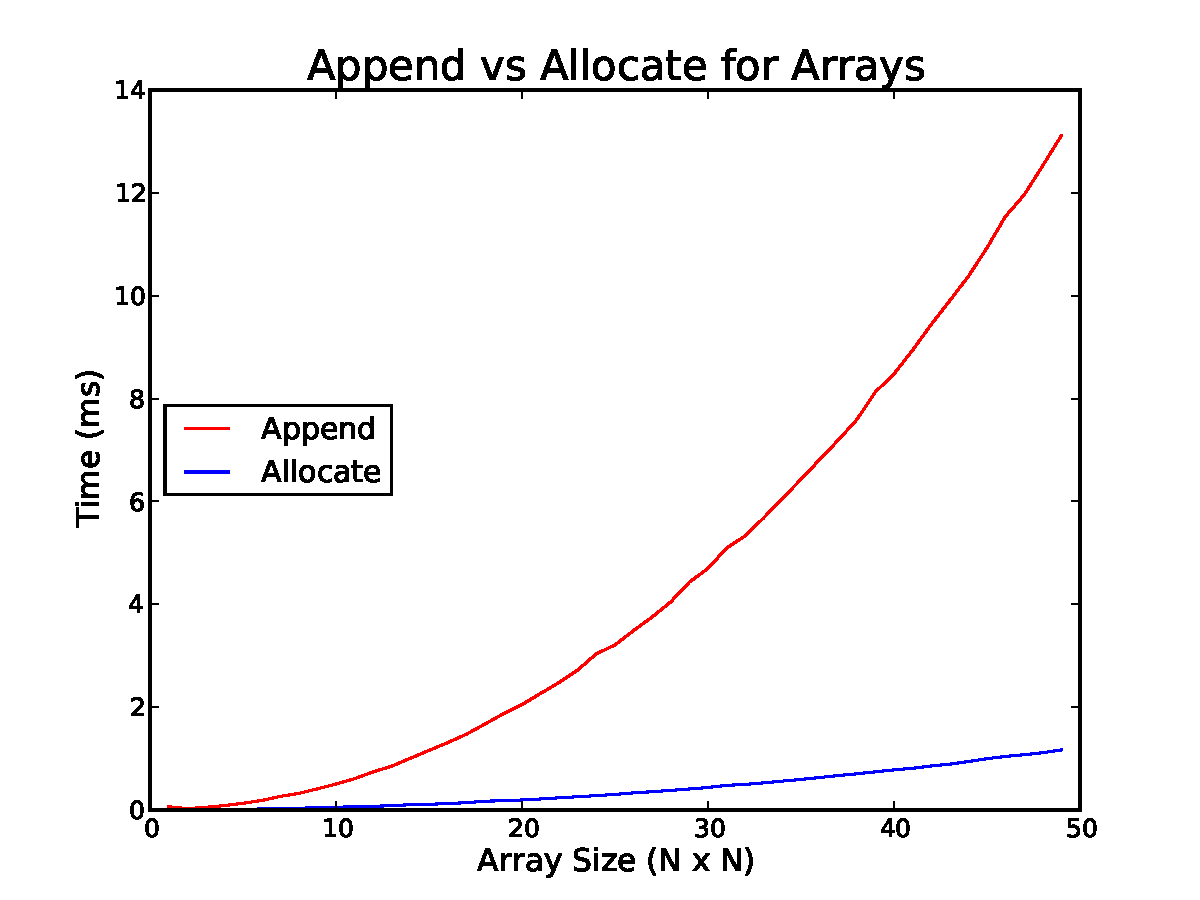
\includegraphics[width=\textwidth]{alloc_vs_resize.pdf}
\end{center}

Why the big difference?  When appending to an array, a new array has to be created with room for the new entry.  Then each element of the old array has to be copied to the new array ending with the new value being inserted at the end of the array.  It is best to allocate space for the final array and change the elements in the array as needed.

\section*{Saving and Loading Arrays}
SciPy allows you to save arrays for later use and load them back again.
\begin{lstlisting}[style=python]
: A = sp.rand(9,9)
: B = sp.random.randint(50, size=(10,10))
: sp.save("testA", A) #saves a single array to a file
: sp.savez("testAB", A = A, B = B) #save multiple arrays to a file
: a = sp.load("testA.npy")
: z = sp.load("testAB.npz")
: z.keys() #the arrays referenced by key
\end{lstlisting}

\begin{problem}
Define a function that will generate an array with the multiplication table for a number, $n$.  Make the function as short and concise as possible.
\end{problem}

\section*{Matplotlib}
Matplotlib is a 2D plotting library for Python that can produce publication quality plots and graphs.  This library provides the visualization component to our numerical computing toolbox.

We import Matplotlib and make it available under the \li{plt} namespace.
\begin{lstlisting}[style=python]
: import matploblib.pyplot as plt
: x = sp.linspace(0, 2*sp.pi)
: plt.plot(x, sp.cos(x))
: plt.show()
\end{lstlisting}

Plotting with Matplotlib works much the same way as plotting with MATLAB.  Many of the command share similar names and accept similar inputs.  For a better idea of what Matplotlib can do, please visit their website at \url{http://matploblib.sourceforge.net}

\section*{Practice}
Let us look at the efficiency of NumPy arrays.  We will do this by implementing the Sieve of Eratosthenes using both arrays and lists.

\begin{problem}
Implement the Sieve of Eratosthenes using Python lists.  Make the implementation 
\end{problem}
